\documentclass[sigconf,anonymous]{aamas}
\usepackage{balance}
\usepackage{algorithm}
\usepackage[noend]{algpseudocode}
\usepackage{tikz}
\usetikzlibrary{arrows.meta,positioning,shapes.geometric,fit,calc,decorations.pathreplacing}
\graphicspath{{vendor/}}
\setlength{\emergencystretch}{2em}

\definecolor{degroblue}{HTML}{3C78A8}
\definecolor{degrogreen}{HTML}{4E9A67}
\definecolor{degroorange}{HTML}{D98C3F}
\definecolor{degrolight}{HTML}{F2F5F8}
\definecolor{degrogray}{HTML}{5A5A5A}

\newcommand{\takeaway}[1]{%
  \par\smallskip
  \noindent\colorbox{degrogray}{\parbox{\dimexpr\columnwidth-2\fboxsep\relax}{\color{white}\bfseries\footnotesize\strut Takeaway}}\par\nointerlineskip
  \noindent\fcolorbox{degrogray}{degrolight}{\parbox{\dimexpr\columnwidth-2\fboxsep-2\fboxrule\relax}{\footnotesize\bfseries\strut #1\strut}}%
  \par\smallskip}

\makeatletter
\gdef\@copyrightpermission{%
  \begin{minipage}{0.2\columnwidth}
  \href{https://creativecommons.org/licenses/by/4.0/}{
\includegraphics[width=.9\textwidth]{by}}
  \end{minipage}\hfill
  \begin{minipage}{0.8\columnwidth}
  \href{https://creativecommons.org/licenses/by/4.0/}{This work is licensed under a Creative Commons Attribution International 4.0 License.}
  \end{minipage}\vspace{5pt}}
\makeatother
\setcopyright{ifaamas}
\acmConference[AAMAS 2027]{Proc. of the 26th International Conference on Autonomous Agents and Multiagent Systems (AAMAS 2027)}{3--7 May 2027}{Hanoi, Vietnam}{M. Baldoni, F. Fang, W. Yeoh, N. Yorke-Smith (eds.)}
\copyrightyear{2027}\acmYear{2027}\acmDOI{}\acmISBN{}
\acmSubmissionID{ANONYMOUS}
\submissionType{Research Paper Track}

\newcommand{\method}{\textsc{DeGro}}

\title{DeGro: Target Determinacy Verification and Grounded Repair for Executable Mathematical Reasoning}
\author{Anonymous Author(s)}

\begin{abstract}
Executable mathematical reasoning may run successfully while solving an underconstrained or mistranslated problem.  Execution checks expose syntax, runtime, and arithmetic failures but do not establish that the encoded constraints determine the requested quantity.  We introduce \emph{DeGro}, a neuro-symbolic framework for \emph{target determinacy diagnosis}.  DeGro asks a solver for two feasible assignments that disagree on the target; when they exist, a grounded policy adds only a source-supported constraint that restores determinacy or abstains.  In a preregistered paired evaluation that fixes the formalization while varying source support, DeGro improves repair-or-abstain accuracy for GPT-OSS 20B but not Gemma 4 31B.  Human-verified natural-error studies show that DeGro improves accuracy on the supported MATH-500 cohort, while higher-coverage ALG514 reveals answer-compatible formalization errors.  Detection is much easier than repair, and concrete witnesses add no measurable benefit beyond the verdict.  Target determinacy is therefore an auditable intermediate guardrail, not a proof of source-to-formal faithfulness.
\end{abstract}
\ccsdesc[500]{Computing methodologies~Knowledge representation and reasoning}
\ccsdesc[500]{Computing methodologies~Intelligent agents}
\ccsdesc[300]{Computing methodologies~Natural language processing}
\keywords{neuro-symbolic reasoning, mathematical agents, verification, counterexamples, abstention}

\begin{document}
\maketitle

\section{Introduction}
Large language models increasingly delegate mathematical computation to programs and symbolic solvers.  Program-aided reasoning reduces arithmetic errors, while systems such as SymCode generate self-contained symbolic programs and repair execution failures~\cite{gao2023pal,nezhad2026symcode}.  Yet successful execution is a weak certificate: it shows that an artifact runs, not that the artifact encodes enough of the source problem to justify the requested answer.

Consider: ``Ten tasks are divided between A and B. A receives two more than B. How many does A receive?''  A generated model containing only $a+b=10$ is executable and satisfiable, but $(a,b)=(4,6)$ and $(6,4)$ imply different values of the target $a$.  The same model is faithful for the shorter source ``Ten tasks are divided between A and B. How many does A receive?''  In the first case, $a=b+2$ is a missing translation; in the second, adding it fabricates information.  The solver state is identical, but the correct action changes with source support.

Execution success, answer agreement, and scalar confidence do not expose whether the feasible region determines the target or whether the source licenses a proposed repair.  A fluent agent may therefore report one value even when its model permits several.

We propose \method{}, a neuro-symbolic framework that treats this failure as structured diagnosis.  It constructs two renamed copies of the generated specification and asks whether both copies can satisfy the constraints while disagreeing on the target.  A satisfying query yields auditable evidence of ambiguity.  DeGro then separates two causes of that ambiguity through a source-grounded repair-or-abstain gate: repair a supported omission, or decline to invent the missing fact.

\begin{figure}[t]
\centering
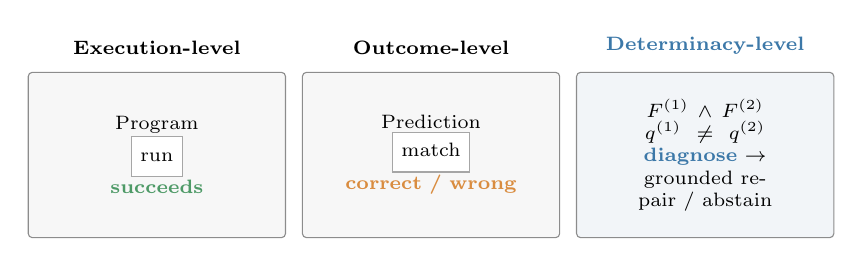
\begin{tikzpicture}[
  panel/.style={draw=black!45,rounded corners=1.5pt,text width=.255\columnwidth,minimum height=21mm,align=center,inner sep=2.5pt,font=\scriptsize},
  tag/.style={font=\scriptsize\bfseries,align=center},
  arrow/.style={-{Latex[length=1.4mm]},semithick}
]
\node[panel,fill=black!3] (exec) {Program\\ \fcolorbox{black!35}{white}{\strut run}\\ \textcolor{degrogreen}{\bfseries succeeds}};
\node[tag,above=1mm of exec] {Execution-level};
\node[panel,fill=black!3,right=2mm of exec] (answer) {Prediction\\ \fcolorbox{black!35}{white}{\strut match}\\ \textcolor{degroorange}{\bfseries correct / wrong}};
\node[tag,above=1mm of answer] {Outcome-level};
\node[panel,fill=degrolight,right=2mm of answer] (diag) {$F^{(1)}\land F^{(2)}$\\ $q^{(1)}\neq q^{(2)}$\\ \textcolor{degroblue}{\bfseries diagnose} $\rightarrow$\\grounded repair / abstain};
\node[tag,above=1mm of diag,text=degroblue] {Determinacy-level};
\end{tikzpicture}
\caption{Three levels of executable-reasoning evaluation.  Execution and outcome checks return coarse judgments; DeGro diagnoses whether feasible models disagree on the requested target and grounds the resulting action in the source.}
\Description{A three-panel comparison of execution-level, outcome-level, and determinacy-level evaluation. The determinacy panel uses two copies of a specification with unequal targets and leads to grounded repair or abstention.}
\label{fig:paradigms}
\end{figure}

Our contributions are: \textbf{(1)} a target-centric property, weaker than full model uniqueness, that matches what an answering agent must justify; \textbf{(2)} a two-copy diagnostic and deterministic gate accepting only source-supported, consistent, non-redundant repairs that restore determinacy; and \textbf{(3)} a preregistered paired evaluation, complemented by human-verified natural errors, that separates repair from abstention and exposes model-dependent gains and a detection--repair gap.  We study decision accuracy (\textbf{RQ1}), unsupported additions (\textbf{RQ2}), witness utility (\textbf{RQ3}), and natural-error coverage, detection, and repair (\textbf{RQ4}).

\section{Related Work}
\paragraph{Executable reasoning and learned verification.}
Chain-of-thought externalizes intermediate reasoning~\cite{wei2022cot}, while PAL and Program-of-Thoughts delegate computation to generated programs~\cite{gao2023pal,chen2023pot}.  Toolformer and ReAct study general tool use~\cite{schick2023toolformer,yao2023react}; MathCoder and ToRA specialize executable actions to mathematics~\cite{wang2024mathcoder,gou2024tora}.  Faithful chain-of-thought further makes symbolic execution part of the rationale~\cite{lyu2023faithful}.  SymCode makes a symbolic program the central reasoning artifact and repairs runtime failures~\cite{nezhad2026symcode}.  These systems improve calculational reliability, but execution success does not imply that the artifact contains enough constraints to justify its requested target.  DeGro addresses this complementary post-generation failure: a program can parse, run, and return a value while its feasible region permits several answers.

Outcome verifiers rank candidate answers, and process supervision evaluates intermediate steps~\cite{cobbe2021verifiers,uesato2022feedback,lightman2023verify}.  Self-verification, Self-Refine, and CRITIC instead ask the model to inspect or revise its own output~\cite{weng2023selfverification,madaan2023selfrefine,gou2024critic}.  Such revision can improve answer accuracy, but intrinsic self-correction is unreliable without an external signal~\cite{huang2024selfcorrect}.  DeGro supplies a mechanical, target-specific signal rather than a scalar score or free-form critique.  Its witness refutes determinacy of the representation; it does not certify a replacement constraint.

\paragraph{Relational diagnosis and repair.}
Self-composition reduces a two-execution property to an ordinary safety query by composing a program with a renamed copy~\cite{barthe2004selfcomposition,terauchi2005safety}.  Product programs and Cartesian Hoare logic make relational arguments modular~\cite{barthe2011product,sousa2016cartesian}, while hyperproperties and HyperLTL generalize reasoning from individual traces to sets of traces~\cite{clarkson2010hyperproperties,clarkson2014hyperltl,finkbeiner2015modelchecking}.  DeGro uses the same two-copy idea for a different relation: agreement on a mathematical target across all feasible assignments.  This query is weaker than full state uniqueness and therefore better aligned with what an answering agent must establish.

Recent symbolic systems diagnose semantic defects that ordinary execution misses.  ReLoop perturbs parameters to expose faulty optimization models that still execute~\cite{lian2026reloop}.  SymDiag performs step-level satisfiability and entailment checks and returns structured evidence~\cite{cui2026symdiag}.  Core-guided methods repair overconstrained formalizations, building on minimal-unsatisfiable-subset analysis~\cite{sarkar2026cores,liffiton2008mus}.  DeGro occupies the underconstrained regime: $F$ is satisfiable, yet two feasible models disagree on $q$.  Its mechanical refutation is related to counterexample-guided abstraction and synthesis~\cite{clarke2000cegar,solarlezama2006cegis} and to failure-inducing-input reduction~\cite{zeller2002simplifying}, but establishes ambiguity rather than revealing the correct edit.

\paragraph{Grounding, abstention, and faithfulness.}
Selective prediction formalizes risk--coverage tradeoffs under a reject option~\cite{elyaniv2010foundations,geifman2017selective,geifman2019selectivenet,cortes2016rejection}, while learning-to-defer routes difficult cases to another decision-maker~\cite{mozannar2020defer} and conformal risk control calibrates selected actions~\cite{angelopoulos2024conformal}.  Language-model self-knowledge and semantic uncertainty provide confidence signals~\cite{kadavath2022know,kuhn2023semantic}.  DeGro instead asks whether the encoded constraints logically permit several target values and whether the source licenses a restriction.  An \textsc{unknown} solver result is a coverage failure, not evidence of ambiguity; an ambiguous target requires repair, clarification, or abstention even when a language model is confident.

Classical diagnosis identifies faulty assumptions, and abduction searches for hypotheses that restore a desired property~\cite{reiter1987diagnosis,dillig2013abduction}.  SAT-based model repair changes a transition system until it satisfies a specification~\cite{attie2008modelrepair}, and LLM-based work repairs declarative Alloy models~\cite{alhanahnah2024alloyrepair}.  Our admissible edit is intentionally narrower: the proposal must cite its source, preserve consistency, add information not already entailed, and restore target determinacy.  This design prevents the trivial ``repair'' of pinning the target to a guessed answer.

Autoformalization and theorem proving provide increasingly capable formal artifacts~\cite{wu2022autoformalization,jiang2024mma,jiang2023draft,yang2023leandojo,azerbayev2024llemma,xin2024deepseekprover}.  Benchmarks including miniF2F, ProofNet, Lean Workbook, and FormalMATH broaden the formal evaluation substrate~\cite{zheng2022minif2f,azerbayev2023proofnet,ying2024leanworkbook,yu2025formalmath}, but prover acceptance alone does not establish preservation of source meaning.  MIRA-Math studies questions requiring a hidden necessary fact~\cite{albateh2026mira}.  We use its validated latent states to construct matched repair and abstention cases while withholding the latent answer from the repair model.  The resulting evaluation focuses on grounded representation repair rather than theorem acceptance or information exchange.

\section{Method}
DeGro is a two-stage framework: it first diagnoses whether a generated specification determines the requested target, then converts an ambiguous verdict into either a source-grounded repair or a principled abstention.  Figure~\ref{fig:workflow} summarizes the complete loop.

\subsection{Problem Setup, Determinacy, and Soundness}
Let a natural-language problem be $P$.  A model produces $F=(V,D,C,q)$, where $V$ are variables, $D$ their domains, $C$ constraints, and $q(V)$ the requested expression.  Define
\[
\mathrm{Sol}(F)=\{m\mid m\models D\land C\}.
\]
The target is \emph{determinate under $F$} iff
\[
\forall m_1,m_2\in\mathrm{Sol}(F),\quad q(m_1)=q(m_2).
\]
This is weaker than solution uniqueness: $x=5,y\geq0$ has many models, but target $q=x$ is determinate.

Construct renamed copies $F^{(1)}$ and $F^{(2)}$ and query
\begin{equation}
\Phi(F,q)=F^{(1)}\land F^{(2)}\land q(V^{(1)})\neq q(V^{(2)}).\label{eq:query}
\end{equation}
If \eqref{eq:query} is satisfiable, its two projected models form a \emph{target-divergent witness pair}.  If it is unsatisfiable and $F$ itself is satisfiable, the target is determinate.

\textbf{Guarantee.} For a sound solver and supported theory, $\mathrm{SAT}(F)$ and an \textsc{unsat} result for Eq.~\eqref{eq:query} imply that all models of $F$ agree on $q$; any disagreeing pair would satisfy the query.  Timeout and \textsc{unknown} prove nothing.  The guarantee is query-relative and strictly about $F$, not semantic equivalence $F\equiv P$: extra or wrong constraints may force a unique but mistranslated answer.  Conversely, arbitrary strengthening can always force determinacy, motivating a separate source-grounding requirement.  The policy therefore adds constraints only to ambiguous specifications; deleting or revising a determinate but wrong representation is outside scope.

Target determinacy is deliberately weaker than model uniqueness.  A scheduling model may leave many assignments free while fixing total cost, and a word problem may admit several assignments to nuisance variables while fixing the requested quantity.  Rejecting such cases would confuse representational freedom with answer ambiguity.  A witness pair is also independently checkable: substitute each assignment into $D\land C$ and compare its target value.  Determinacy is monotone under consistent strengthening, but the converse is unsafe because an arbitrary fact such as $q=6$ can always collapse the feasible target set.

\paragraph{Running example.}
Let $V=\{a,b\}$ be nonnegative integers, $C=(a+b=10)$, and $q=a$.  The duplicated query can return $(a_1,b_1)=(4,6)$ and $(a_2,b_2)=(6,4)$.  If $P$ says ``A receives two more than B,'' then $a=b+2$ is supported, consistent, non-redundant, and sufficient, yielding $a=6$.  Without that sentence, the same equation is a fabricated assumption and the correct action is abstention.  The repair model sees neither the hidden gold value nor the missing gold constraint.

\paragraph{Structured representation.}
The agent emits one typed \textsc{ModelSpec} with variable sorts and bounds, source-linked constraints, and a target.  Deterministic compilers translate it to computational and verification backends, avoiding independently generated SymPy and SMT programs.  The supported fragment covers integer, real, and Boolean variables, arithmetic equalities and inequalities, finite domains, and selected modular constraints; other syntax yields \textsc{not-supported}.

\subsection{Stage I: Target-Determinacy Diagnosis}
DeGro first tests $\mathrm{SAT}(F)$, returning \textsc{inconsistent} or \textsc{unknown} when appropriate, and otherwise evaluates Eq.~\eqref{eq:query}.  Unsatisfiability permits an answer under $F$; satisfiability returns two assignments with different targets and triggers repair.  This stage is deterministic: the model proposes $F$ but does not judge determinacy.

\begin{algorithm}[H]
\caption{Target-determinacy verification}
\label{alg:verify}
\footnotesize
\begin{algorithmic}[1]
\Require Typed specification $F=(V,D,C,q)$
\Ensure Status and optional witness pair
\State $r_0 \gets \Call{CheckSat}{D\land C}$
\State \textbf{if} $r_0=\textsc{unsat}$ \textbf{return} \textsc{inconsistent}
\State \textbf{if} $r_0\neq\textsc{sat}$ \textbf{return} \textsc{unknown}
\State $\Phi\gets F^{(1)}\land F^{(2)}\land(q^{(1)}\neq q^{(2)})$ using disjoint copies
\State $(r_1,M) \gets \Call{CheckSat}{\Phi}$
\State \textbf{if} $r_1=\textsc{unsat}$ \textbf{return} \textsc{determinate}
\State \textbf{if} $r_1\neq\textsc{sat}$ \textbf{return} \textsc{unknown}
\State \Return $\textsc{ambiguous},\Call{ProjectWitnesses}{M}$
\end{algorithmic}
\end{algorithm}

The record stores both solver verdicts, normalized target values, and complete witnesses when available.  Only \textsc{ambiguous} licenses repair; unsupported theories and timeouts are never coerced into Boolean outcomes.

\subsection{Stage II: Grounded Repair or Abstention}
The repair model receives $P,C,q$ and the witness pair, then returns \textsc{add-constraint} with an exact supporting span or \textsc{abstain}.  A candidate must compile, cite text in $P$ (or a declared domain rule), preserve satisfiability, be non-redundant, and restore determinacy.  DeGro uses at most two rounds and otherwise returns \textsc{underspecified}.  Exact-span provenance is auditable but does not prove that the cited text was translated correctly.

The witness is diagnostic rather than corrective: it identifies a disagreement but does not reveal which missing relation the source licenses.  The language model proposes that relation, and the deterministic gate decides whether it can enter the trusted specification.  If an accepted addition yields a new divergent pair instead of determinacy, the second and final round receives the updated diagnosis.  A rejected proposal never partially mutates $F$.  Thus the loop is bounded and rollback-free, unlike unconstrained self-refinement whose successive edits may obscure their evidential basis.

\subsection{Trusted Implementation and Repair Semantics}
The implementation compiles a restricted expression AST to Z3~\cite{demoura2008z3}, rejecting arbitrary calls, undeclared names, malformed comparisons, and unsupported operators.  Independent variable maps prevent aliasing between copies.  Grounding is a deterministic deployment gate, not a prompt instruction; raw proposals and gated outcomes are both retained.  The trusted base is the parser, compiler, solver, and gate, while the language model remains untrusted.

Integer, real, and Boolean declarations are typed explicitly, and declared bounds compile into constraints.  The computational and verification backends consume the same normalized \textsc{ModelSpec}; independently generated Python and SMT artifacts could otherwise disagree while both appear valid.  Every record stores the initial verdict, proposed action, cited span, rejection reason, final verdict, model configuration, and prompt hash.  This audit trail separates model behavior from enforcement behavior.

\paragraph{Repair acceptance.}
Let $\mathrm{span}(c)$ be the source substring cited for candidate $c$, and let $\mathcal{R}$ be a frozen set of allowed domain-semantics rules.  The gate accepts $c$ exactly when
\begin{align}
\mathrm{Accept}(c) \iff{}& \mathrm{Compiles}(c) \land
  \mathrm{Grounded}(c,P,\mathcal{R}) \nonumber\\
&\land\ \mathrm{SAT}(F\land c) \land \neg(F\models c)
  \land \mathrm{Det}(F\land c,q),
\label{eq:accept}
\end{align}
where grounding requires an exact source span or named rule in $\mathcal{R}$.  The first accepted candidate is committed; otherwise $F$ is preserved.  Thus redundant restatements, unsupported target pins, and insufficient additions cannot receive repair credit, while a supported expression need not match the gold syntax.

\paragraph{Complexity and failure states.}
Encoding size is linear in $|F|$, although solver time depends on the theory.  A determinate input needs no repair call; an ambiguous one incurs at most two calls plus rechecks.  We preserve distinct states: \textsc{unsupported} for representation limits, \textsc{unknown} for solver inconclusiveness, \textsc{inconsistent} for an unsatisfiable $F$, and \textsc{underspecified} when an ambiguous target lacks a grounded repair.

These states have different controller implications.  An unsupported construct should route to another tool or a broader compiler; an unknown query may warrant a larger solver budget; an inconsistent model requires revising the encoding; and an underspecified source should trigger clarification or abstention.  Collapsing all four into ``failure'' would make both coverage reporting and agent behavior uninterpretable.  Likewise, a determinate verdict authorizes only an answer scoped to $F$, not an assertion that the source has been fully formalized.

\begin{figure*}[t]
\centering

\includegraphics[width=.82\textwidth]{figure/pipeline.jpg}
\caption{DeGro in the executable-reasoning pipeline.  SymCode generates the executable artifact, while DeGro passes a structured \textsc{ModelSpec} to Z3-backed target-determinacy verification.  A determinate target can be answered, an ambiguous target enters grounded repair and validation, and an inconclusive check returns no certificate.}
\Description{A pipeline from a mathematical problem through SymCode generation and Python code to DeGro. DeGro verifies a structured ModelSpec with Z3 and routes determinate, ambiguous, and no-verdict outcomes to answer, grounded repair or abstention, and no certificate, respectively.}
\label{fig:workflow}
\end{figure*}

\subsection{Agent Integration and Controller Semantics}
DeGro is a verifier policy inside a larger agent.  It converts an executable artifact into a typed observation that the controller maps to an action (Table~\ref{tab:policy}).

\begin{table}[t]
\centering
\caption{Controller semantics for DeGro integration.}
\label{tab:policy}
\small
\begin{tabular}{lll}
\toprule
Verifier state & Evidence & Controller action\\
\midrule
Determinate & $F$ sat, $\Phi$ unsat & answer with scope\\
Ambiguous & targets disagree & grounded repair\\
Inconsistent & $F$ unsat & revise encoding\\
Unknown & solver inconclusive & fallback/escalate\\
Unsupported & outside fragment & alternate tool\\
Underspecified & no grounded repair & ask or abstain\\
\bottomrule
\end{tabular}
\end{table}

In interactive use, \textsc{underspecified} can request clarification; the benchmark scores abstention because no information channel exists.  Separating generation, deterministic verification, and repair reduces self-confirmation and yields an audit trail.  Interfaces should report that ``the encoded constraints determine the target,'' not that the source problem was formally proved.

\section{Experiments and Results}
\subsection{Experimental Setup}
\paragraph{Controlled paired benchmark.}
For each gold specification $F^*=\{c_1,\ldots,c_k,c^*\}$, we form $F^-=F^*\setminus\{c^*\}$ and retain it only if $F^*$ determines the target while $F^-$ is satisfiable and target-ambiguous.  Each pair shares $F^-$: an \textsc{omission} source contains the fact for $c^*$ and requires repair, whereas an \textsc{underspecified} source omits it and requires abstention.  The verifier state alone therefore cannot reveal the label.  After excluding an 80-pair pilot and 100-pair development set, we froze 120 confirmatory MIRA-Math pairs (240 cases, five families)~\cite{albateh2026mira}; the combined 300-pair analysis is secondary.

\paragraph{Integrity checks.}
The builder imports the typed missing fact from MIRA-Math rather than asking an LLM to corrupt the problem, then applies all three solver checks.  The final set exhausts compatible unseen identifiers; its manifest records source revision \texttt{72ff918}, license, selection seed, family counts, and prompt/output hashes.  The five families cover linear separation, rank-deficient systems, path sums, Chinese-remainder reconstruction, and moment constraints.

The families exercise distinct structures.  Linear separation removes a relation that distinguishes otherwise compatible solutions; rank-deficient systems preserve several degrees of freedom.  Graph path sums and Chinese-remainder reconstruction combine discrete equalities with domain restrictions, while moment problems couple polynomial summaries within the supported degree bound.  Family-stratified results check that one easy template does not dominate the aggregate.  Because every retained deletion is mechanically verified as target-critical, the benchmark does not mislabel an irrelevant omission as a repair opportunity.

\paragraph{Methods and hypotheses.}
We compare \textsc{self-review}, \textsc{grounded self-review}, \textsc{determinacy-guided repair}, and \textsc{DeGro} under the same initial formalization and two-attempt budget.  GPT-OSS 20B and Gemma 4 31B use medium reasoning, temperature 1.0, and frozen prompts; all $120\times2\times4=960$ records per model are present.  A disjoint 100-pair exploratory study compares verdict-only and witness variants for RQ3.

Self-review receives the executable artifact and asks for correction without formal diagnosis.  Grounded self-review adds the same source-citation requirement used by DeGro.  Determinacy-guided repair supplies the typed solver verdict but no grounding interaction, isolating the diagnostic signal.  DeGro combines that signal with source evidence and applies the same deterministic acceptance gate used in scoring.  Since all methods begin from an identical $F^-$, differences cannot be attributed to initial-generation quality.

The preregistered primary comparison tests whether DeGro improves FDA over grounded self-review.  We test it separately for each model with exact paired McNemar tests and Holm correction across the two tests.  We report the paired percentage-point difference with a pair-cluster bootstrap 95\% interval.  Official model documentation describes configurable reasoning effort and structured output support for GPT-OSS~\cite{openai2025gptoss}.

\paragraph{Metrics and analysis.}
Repair success rate (RSR) requires a grounded, functionally correct addition; correct abstention rate (CAR) rewards abstention on underspecified cases.  Final decision accuracy (FDA) averages the balanced case types, over-repair rate is $1-\mathrm{CAR}$, and unsupported repair (UR) is the share of additions lacking source support.  Pair-cluster confidence intervals preserve within-pair dependence; semantic, functional, and grounded outcomes remain separate.

\paragraph{Natural-error study.}
For ecological validity, GPT-OSS 20B generated one Structured SymCode specification per MATH-500 problem without injected errors.  We froze all parsed, solver-supported, conclusive cases before annotation or outcome inspection and reused each initial specification across methods.  Model-proposed labels and evidence were hidden from verifier outputs, then fully checked by two reviewers: all 292 MATH-500 and 503 ALG514 cases.  Because separate pre-discussion human labels were not retained, we claim human verification, not independent annotation or inter-annotator agreement.  Labels distinguish correct, missing/wrong/extra constraint, wrong domain, wrong target, computational error, and other; only source-supported target-critical omissions enter the primary subset.

For MATH-500, GPT-OSS 20B and Gemma 4 31B first proposed labels under a shared prompt while blinded to determinacy, witnesses, repairs, and method outcomes.  Reviewers inspected all 292 Gemma-proposed labels and accepted the adjudicated result.  For ALG514, GPT-OSS 120B proposed 503 labels and re-adjudicated all 22 cases where semantic status disagreed with verifier-compatible numerical status; reviewers then inspected all final labels.  Detector ambiguity could not define the positive class: a positive required a source-supported omission that can change the requested target.

Primary natural-error measures are ambiguity recall and end-to-end grounded repair; secondary measures include precision, false ambiguity/repair, and preservation of correct controls.  Proportions use Wilson 95\% intervals and paired answer accuracy uses exact McNemar.  Numeric agreement alone is not repair success.

The original problem is the unit of analysis, and every method reuses its shared initial formalization.  Recall asks how often DeGro identifies verified target-critical omissions; precision asks how often an ambiguous verdict corresponds to that class.  Conditional repair counts accepted grounded fixes among detected omissions, whereas end-to-end repair retains every verified omission in the denominator.  This distinction exposes the gap between finding ambiguity and recovering the missing source relation.

MATH-500 contributes 292 of 500 conclusive, solver-supported formalizations; ALG514 contributes 503 of 514.  Exclusions are reported in the coverage results.  DRAW-1K is omitted because corrected-verifier outcomes and final human labels were incomplete.

\subsection{Results}
Table~\ref{tab:main} reports the preregistered 120-pair analysis.  For GPT-OSS 20B, DeGro raises FDA from 90.0\% to 95.0\% relative to grounded self-review, a $+5.0$-point effect (95\% CI $[0.4,9.6]$; discordant counts 22 versus 10; exact McNemar $p=.050$, Holm $p=.100$).  For Gemma 4 31B, FDA changes from 97.9\% to 97.5\%, a $-0.4$-point effect (95\% CI $[-3.3,2.5]$; 5 versus 6; $p=1.0$).  Thus the confirmatory result supports a practically meaningful GPT-OSS gain but not a model-general advantage.  The strongest Gemma result is the verdict-only determinacy method (99.6\% FDA), showing that the additional grounding interaction can itself introduce errors.

\begin{table}[t]
\centering
\caption{Confirmatory results on 120 preregistered pairs per model.  UR is unsupported additions divided by all proposed additions.}
\label{tab:main}
\resizebox{\columnwidth}{!}{%
\begin{tabular}{llrrrrr}
\toprule
Model & Method & RSR$\uparrow$ & CAR$\uparrow$ & FDA$\uparrow$ & ORR$\downarrow$ & UR$\downarrow$\\
\midrule
GPT-OSS & Self-review & 93.3 & 87.5 & 90.4 & 12.5 & 15.2\\
20B & Grounded self-review & 100.0 & 80.0 & 90.0 & 20.0 & 16.7\\
 & Determinacy-guided & 86.7 & 99.2 & 92.9 & 0.8 & 6.3\\
 & DeGro & 92.5 & 97.5 & \textbf{95.0} & 2.5 & 4.3\\
\midrule
Gemma 4 & Self-review & 100.0 & 93.3 & 96.7 & 6.7 & 6.3\\
31B & Grounded self-review & 100.0 & 95.8 & 97.9 & 4.2 & 4.0\\
 & Determinacy-guided & 100.0 & 99.2 & \textbf{99.6} & 0.8 & 0.8\\
 & DeGro & 100.0 & 95.0 & 97.5 & 5.0 & 4.8\\
\bottomrule
\end{tabular}
}
\end{table}

\paragraph{Secondary cumulative analysis.} Across all 300 pairs, DeGro versus grounded self-review changes FDA from 91.2\% to 96.2\% for GPT-OSS (difference $+5.0$ points, 95\% CI $[2.3,7.7]$; McNemar $p<.001$) and from 96.2\% to 97.8\% for Gemma (difference $+1.7$ points, 95\% CI $[-0.2,3.5]$; $p=.099$).  These cumulative estimates include development data and do not replace the 120-pair confirmatory tests.

\paragraph{Human-verified natural errors.}
On the supported MATH-500 cohort, 158 of 292 formalizations are correct; the remaining labels are 69 wrong-target, 32 wrong-constraint, 24 target-critical missing-constraint, eight extra-constraint, and one wrong-domain.  The detector identifies 21 of 24 target-critical omissions (87.5\% recall, 95\% Wilson CI $[69.0,95.7]$) but precision is 17.4\% ($21/121$), and only one omission is successfully repaired end to end ($1/24=4.2\%$).  DeGro nevertheless raises cohort answer accuracy from 49.3\% ($144/292$) to 53.8\% ($157/292$); 16 discordant cases favor DeGro and three favor the structured baseline (exact McNemar $p=.0044$).  This prevalence is conditional on 58.4\% solver-fragment coverage.

ALG514~\cite{upadhyay2017derivations} provides a higher-coverage contrast: 503 of 514 cases enter the verified cohort, of which 477 are correct, 11 wrong-target, eight missing-constraint, and seven wrong-constraint.  The semantic-error rate is 5.2\% (95\% Wilson CI $[3.6,7.5]$).  Structured Solver and DeGro score 94.2\% ($484/514$) and 94.4\% ($485/514$), respectively, using order-invariant subset matching with $10^{-3}$ tolerance for ALG514's all-unknown, rounded solution vectors.  Nine numerically compatible answers retain a human-verified semantic error, directly showing that answer-only evaluation can conceal representation failures.  The one-case DeGro gain on ALG514 is exploratory.

\paragraph{Detection--repair decomposition.}
The natural-error results separate three questions that an aggregate answer score conflates.  First, representation coverage asks whether the structured language and solver can express and decide the generated model.  Second, ambiguity detection asks whether target-divergent assignments exist within that model.  Third, grounded repair asks whether the original source supports a new constraint that removes the disagreement.  MATH-500 performs moderately on the first stage (292 of 500), strongly on recall at the second (21 of 24 omissions), and poorly on the third (one of 24).  The bottleneck is therefore not simply detecting non-uniqueness; it is converting a solver counterexample into a semantically correct, cited edit.

Precision provides the complementary view.  Only 21 of 121 ambiguous MATH-500 specifications are verified target-critical omissions.  The remaining ambiguous cases include wrong targets, wrong constraints, and representations whose feasible set is broad for reasons other than a missing source fact.  These are legitimate warnings about $F$ but not opportunities for additive repair.  A high-recall detector can consequently be useful for routing while still requiring a strict gate: automatically treating every ambiguity as an omission would reproduce the over-repair behavior observed in generic self-review.

Answer accuracy alone also understates the semantic distinction.  On MATH-500, DeGro changes the shared structured baseline from 49.3\% to 53.8\%, with 16 discordances favoring DeGro and three favoring the baseline.  Yet only one verified omission is repaired end to end, so most accuracy changes do not constitute evidence that the missing-relation mechanism was solved.  On ALG514, nine numerically compatible outputs still carry a verified semantic defect.  We therefore report numerical, semantic, functional, grounding, and determinacy outcomes separately rather than reinterpret every answer improvement as representation repair.

\paragraph{Decision-theoretic reading.}
FDA assigns equal mass to repair on complete sources and abstention on underspecified sources because every controlled item contributes one of each.  Real applications may penalize fabrication more heavily than missed repair.  The case-level release permits alternative utilities, but the qualitative tradeoff is already visible: generic grounded review attains high RSR while over-repairing, whereas a bare determinacy verdict favors abstention.  DeGro attempts to recover useful repairs without surrendering the conservative action boundary.  Whether that balance is preferable depends on the downstream cost of an unsupported assertion, which should be declared rather than hidden inside a single accuracy metric.

\begin{figure*}[t]
\centering
\begin{minipage}[t]{.47\textwidth}
\centering
\textbf{(a) Confirmatory final decision accuracy}\par\smallskip
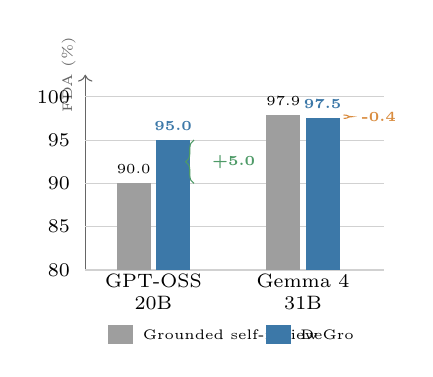
\begin{tikzpicture}[x=1cm,y=1cm,font=\scriptsize]
  \draw[->,black!60] (.45,0) -- (.45,2.48) node[above,rotate=90,anchor=south,font=\tiny]{FDA (\%)};
  \foreach \lab/\yy in {80/0,85/.55,90/1.10,95/1.65,100/2.20}{
    \draw[black!18] (.45,\yy) -- (4.25,\yy);
    \node[anchor=east] at (.38,\yy) {\lab};
  }
  \fill[black!38] (.85,0) rectangle (1.28,1.10);
  \fill[degroblue] (1.35,0) rectangle (1.78,1.65);
  \fill[black!38] (2.75,0) rectangle (3.18,1.969);
  \fill[degroblue] (3.25,0) rectangle (3.68,1.925);
  \node[above,font=\tiny] at (1.065,1.10) {90.0};
  \node[above,font=\tiny,text=degroblue] at (1.565,1.65) {\bfseries 95.0};
  \node[above,font=\tiny] at (2.965,1.969) {97.9};
  \node[above,font=\tiny,text=degroblue] at (3.465,1.925) {\bfseries 97.5};
  \node[align=center] at (1.315,-.28) {GPT-OSS\\20B};
  \node[align=center] at (3.215,-.28) {Gemma 4\\31B};
  \node[draw=black!38,fill=black!38,minimum width=3mm,minimum height=2mm,label={[font=\tiny]right:Grounded self-review}] at (.9,-.82) {};
  \node[draw=degroblue,fill=degroblue,minimum width=3mm,minimum height=2mm,label={[font=\tiny]right:DeGro}] at (2.9,-.82) {};
  \draw[decorate,decoration={brace,amplitude=3pt},degrogreen] (1.83,1.10) -- (1.83,1.65) node[midway,right=3pt,font=\tiny,text=degrogreen]{\bfseries +5.0};
  \draw[decorate,decoration={brace,amplitude=3pt},degroorange] (3.73,1.969) -- (3.73,1.925) node[midway,right=3pt,font=\tiny,text=degroorange]{\bfseries -0.4};
\end{tikzpicture}
\end{minipage}\hfill
\begin{minipage}[t]{.49\textwidth}
\centering
\textbf{(b) MATH-500 diagnostic funnel}\par\smallskip
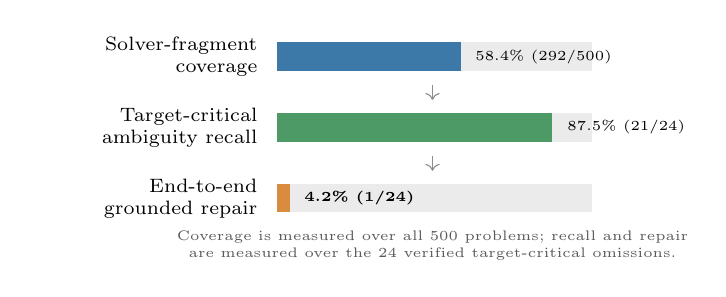
\begin{tikzpicture}[font=\scriptsize]
  \node[anchor=east,align=right,text width=28mm] at (0,2.15) {Solver-fragment\\coverage};
  \node[anchor=east,align=right,text width=28mm] at (0,1.25) {Target-critical\\ambiguity recall};
  \node[anchor=east,align=right,text width=28mm] at (0,.35) {End-to-end\\grounded repair};
  \foreach \yy in {2.15,1.25,.35}{\fill[black!8] (0.12,\yy-.18) rectangle (4.12,\yy+.18);}
  \fill[degroblue] (0.12,1.97) rectangle (2.456,2.33);
  \fill[degrogreen] (0.12,1.07) rectangle (3.62,1.43);
  \fill[degroorange] (0.12,.17) rectangle (.288,.53);
  \node[anchor=west,font=\tiny] at (2.52,2.15) {58.4\%  (292/500)};
  \node[anchor=west,font=\tiny] at (3.69,1.25) {87.5\%  (21/24)};
  \node[anchor=west,font=\tiny] at (.35,.35) {\bfseries 4.2\%  (1/24)};
  \draw[->,black!45] (2.1,1.79) -- (2.1,1.60);
  \draw[->,black!45] (2.1,.89) -- (2.1,.70);
  \node[align=center,font=\tiny,text=black!65] at (2.1,-.25) {Coverage is measured over all 500 problems; recall and repair\\are measured over the 24 verified target-critical omissions.};
\end{tikzpicture}
\end{minipage}
\caption{Two complementary views of the evidence.  (a) DeGro improves confirmatory FDA by five points for GPT-OSS 20B but not for Gemma 4 31B; the axis begins at 80\% to make the paired differences visible.  (b) Natural-error evaluation has a pronounced detection--repair gap: most target-critical omissions are detected, but only one is repaired end to end.}
\Description{Panel a is a grouped bar chart comparing grounded self-review and DeGro final decision accuracy for GPT-OSS 20B and Gemma 4 31B. Panel b shows three horizontal bars for MATH-500 solver-fragment coverage, ambiguity recall, and end-to-end repair success, with counts and denominators.}
\label{fig:result_summary}
\end{figure*}

\paragraph{Witness ablation.}
On the exploratory 100-pair set, DeGro scores 98.5 FDA versus 97.5 with witnesses (five versus three discordances favoring DeGro; Holm-adjusted $p=.727$).  A minimal witness raises RSR by six points over a bare verdict, also non-significantly ($p=.714$).  Concrete assignments therefore add no measurable benefit here: the typed verdict can be exposed by default and witnesses retained for audit or harder cases.

\begin{table}[t]
\centering
\caption{Exploratory GPT-OSS 20B ablation on 100 development pairs.}
\label{tab:ablation}
\small
\begin{tabular}{lrrrr}
\toprule
Method & RSR & CAR & FDA & ORR\\
\midrule
Self-review & 92 & 84 & 88.0 & 16\\
Bare non-uniqueness & 87 & 97 & 92.0 & 3\\
Minimal witness & 93 & 93 & 93.0 & 7\\
Target witnesses & 86 & 94 & 90.0 & 6\\
Minimal witness+ground & 97 & 99 & 98.0 & 1\\
DeGro & 97 & 100 & \textbf{98.5} & 0\\
DeGro+witnesses & 97 & 98 & 97.5 & 2\\
\bottomrule
\end{tabular}
\end{table}

This negative result narrows the contribution.  Every controlled instance contains one target-critical omission, so non-uniqueness already localizes the relevant defect; witness assignments add tokens but little new information.  Specifications with several missing facts or many nuisance dimensions may differ, but these data support determinacy-guided grounding, not a universal benefit from exposing concrete assignments.

\paragraph{Error patterns and cross-model behavior.}
GPT-OSS generic review repairs over 92\% of omissions on the cumulative set but achieves at most 87\% CAR.  A bare verdict raises CAR to 98\% while lowering RSR to 87.7\%; DeGro restores repairs, preserves 99\% CAR, and reduces unsupported additions from 12.5\% to 3.4\% relative to grounded self-review.  Gemma repairs every omission; its bare verdict reaches 99.0 FDA while DeGro reaches 97.8, with unsupported-addition rates of 2.0\% and 4.2\%.  Family effects are concentrated: GPT gains 20.8 points on linear separation but DeGro reaches only 87.5\% on rank-deficient systems.  The aggregate effect is therefore neither uniform nor model-independent.

\begin{table}[t]
\centering
\caption{Cumulative FDA by family for grounded self-review (GSR) and DeGro. Each family contains 60 pairs.}
\label{tab:family}
\small
\begin{tabular}{lrrrr}
\toprule
& \multicolumn{2}{c}{GPT-OSS 20B} & \multicolumn{2}{c}{Gemma 4 31B}\\
Family & GSR & DeGro & GSR & DeGro\\
\midrule
CRT reconstruction & 100.0 & 99.2 & 100.0 & 100.0\\
Graph path sums & 96.7 & 99.2 & 99.2 & 100.0\\
Linear separation & 76.7 & 97.5 & 85.8 & 90.8\\
Moment problem & 88.3 & 97.5 & 98.3 & 100.0\\
Rank-deficient shared & 94.2 & 87.5 & 97.5 & 98.3\\
\bottomrule
\end{tabular}
\end{table}

Table~\ref{tab:family} explains how similar aggregate scores can arise from different mechanisms.  Generic GPT review often inserts a plausible but unstated relation in linear-separation cases; DeGro blocks most of these additions.  In rank-deficient systems, however, the same signal encourages abstention even when the complete source supports repair.  Gemma is near ceiling in four families and has little headroom.  A single average would hide both the beneficial and adverse regimes.

\paragraph{Broad-benchmark coverage audit.}
To measure the representation bottleneck preceding verification, GPT-OSS 20B generated one shared Structured SymCode specification for each MATH-500 problem~\cite{hendrycks2021math}.  Of 500 specifications, 292 (58.4\%) parsed, reached the solver, and produced a conclusive verdict; Table~\ref{tab:coverage} accounts for every exclusion.

\begin{table}[t]
\centering
\caption{Frozen MATH-500 cohort accounting for the shared initial structured specification.}
\label{tab:coverage}
\small
\begin{tabular}{lrr}
\toprule
Disposition & Count & Percent\\
\midrule
Conclusive and solver-supported & 292 & 58.4\\
Model-level unsupported & 65 & 13.0\\
Solver-level unsupported & 112 & 22.4\\
Inconsistent & 9 & 1.8\\
Solver unknown & 9 & 1.8\\
Call error & 13 & 2.6\\
\midrule
Total & 500 & 100.0\\
\bottomrule
\end{tabular}
\end{table}

Coverage is fixed solely from parsing and solver state, not observed answers.  Solver-level unsupported cases dominate and require a broader theory or compiler; model-level failures instead require better structured generation.  Conditional accuracy concerns the 292 supported problems, whereas end-to-end accuracy assigns failures to the other 208.  All Structured Solver records completed; DeGro completed 285, with six call errors and one unsupported record.  We retain the frozen denominator and count all seven as incorrect.

This separation prevents a favorable post-hoc coverage slice.  Conditional accuracy asks how well the agent performs once a specification reaches a conclusive solver state; end-to-end accuracy additionally charges every representation and execution failure.  Reporting only the former would make a narrow verifier appear competitive with unrestricted program generation while hiding 41.6\% of the benchmark.  The exclusion categories also route improvements to the right component: unsupported solver constructs call for broader compilation, while failures before a valid \textsc{ModelSpec} call for better structured generation.

\subsection{Discussion and Limitations}
\paragraph{Interpretation and validity.}
The paired design holds latent values, target, domains, retained constraints, and solver verdict fixed; only the source support for $c^*$ changes.  The repair policy never receives $c^*$, the gold target, or the gold action.  The 120 confirmatory pairs were frozen before inspection, with tests and Holm correction declared in the manifest.  The cumulative analysis remains secondary and the witness ablation exploratory.  FDA equally weights repair and correct abstention; UR must be interpreted with RSR and CAR because always abstaining produces zero unsupported additions but no repair utility.

A conventional mixture of complete and incomplete questions admits shortcuts: families may differ in difficulty, wording may reveal that a fact is missing, and a policy may simply learn to repair every ambiguous solver state.  Our paired construction rules out these shortcuts because both members share the same formalization and diagnostic.  Correct behavior changes only with the natural-language support for the withheld constraint.  Exact McNemar tests then depend only on pairs for which the two policies disagree, while pair-cluster bootstrap intervals preserve the dependence between the two case types.

The primary contrast also controls the language-model interface.  Both methods receive the same source, specification, output schema, grounding instruction, model, and token budget; the added determinacy signal is the intended treatment.  Gold latent values are used only after generation for scoring.  A direct target pin is considered unsupported unless a source span licenses it and all semantic, functional, and determinacy gates accept it.  Retaining raw and gated outputs reveals when apparent accuracy is purchased by fabrication.

\paragraph{Scope of the claim.}
The evidence supports target determinacy as a guard against plausible but unstated repairs, including a five-point GPT-OSS gain.  It does not establish semantic equivalence between $P$ and $F$, a universal grounding benefit, an incremental witness benefit, or superiority over unrestricted code generation.  Exact spans are auditable provenance rather than semantic entailment.  Confidence and determinacy are complementary: low confidence may justify fallback for a determinate target, while confidence cannot authorize an ambiguous one.

The distinction is important for agent design.  An execution monitor answers whether an artifact runs; an outcome verifier may check a final answer; DeGro instead characterizes the feasible set before the agent commits to a value.  This intermediate certificate supports selective action: answer when the target is determined, repair only when a cited source fact restores determinacy, and otherwise ask, abstain, or escalate.  It is not a proof that the formalization matches the source.  A correctly solved but incorrectly translated model may remain determinate.

Grounding itself is also only a proxy.  A model can cite the correct sentence yet encode the wrong equation, while an implicit mathematical convention may justify an expression without a contiguous span.  We therefore keep semantic validity, functional validity, provenance, and solver determinacy as separate fields.  This decomposition makes disagreement auditable and prevents numerical answer correctness from silently absorbing translation errors.

\paragraph{External validity.}
MIRA cases are controlled but templated; MATH-500 is natural but only 58.4\% lies inside the present solver fragment, whereas ALG514 reaches 97.9\% coverage in a narrower domain.  Labels were human-verified after model proposals, not independently annotated, and dataset prevalence is therefore reported separately.  Natural errors contain only 24 MATH-500 and eight ALG514 target-critical omissions: detection is high but repair remains limited.  GPT-OSS and Gemma also differ, directly bounding any model-general claim.

The controlled benchmark deliberately removes one known fact and therefore estimates a clean repair-versus-abstain decision under idealized representation control.  It underrepresents paraphrase, irrelevant prose, diagrams, implicit conventions, wrong constraints, and interacting translation errors.  The natural cohorts contain these phenomena but trade away causal control.  Their purposes are complementary: the paired benchmark identifies a policy effect, while the natural study estimates what the current pipeline actually encounters.  We do not merge them into one leaderboard number.

The annotation protocol also avoids defining positives with DeGro's own verdict.  Detector outputs, repairs, method names, and downstream answer outcomes are hidden from the initial packet.  A target-critical omission must instead be established from the source and generated specification; correct, wrong-constraint, wrong-target, and wrong-domain cases remain in the denominator.  Because model proposals seeded review and no separate blinded pre-discussion labels were preserved, we claim human verification rather than independent annotation or inter-annotator reliability.

\paragraph{Reproducibility and risk.}
The artifact includes the compiler, two-copy query, gates, tests, builders, frozen manifests, prompts, raw records, and analysis.  The confirmatory output hash is \texttt{5616d0c6\ldots4ce3f0b}, and each model analysis consumes all 960 expected records.  Determinacy remains relative to $F$: wrong or extra constraints may force a unique wrong target, non-target omissions are invisible, and the current SMT fragment excludes much nonlinear, transcendental, and diagrammatic reasoning.  Interfaces must expose this scope rather than imply truth.  The data contain no personal information; AI assistance requires venue-compliant disclosure and does not reduce author responsibility.

The manifests record dataset revision and license, selection seed, family counts, exact model strings, decoding settings, prompt hashes, timestamps, and full output hashes.  Analysis scripts reconstruct every table from JSONL, reject incomplete expected pair counts, and preserve whether a row came from pilot, development, or confirmatory data.  Natural-error packets and verified labels are separately blinded and content-addressed.  These records allow the 120-pair headline to be reproduced without incorporating earlier observations.

Several failure modes remain outside the certificate.  A wrong or extra constraint may force a unique but incorrect target; an omitted fact that does not affect $q$ is invisible; several interacting omissions may exceed the bounded repair budget; and witnesses may differ only on irrelevant variables.  The supported SMT fragment excludes much nonlinear, transcendental, and diagrammatic mathematics.  These are reasons to surface the encoded constraints, cited repair, and solver status in the interface, not to display an unqualified ``verified'' badge.

Finally, the two models exhibit different instruction-following and abstention behavior, and hosted checkpoints may change.  DeGro's advantage should therefore be treated as a property of a specified model--prompt--gate configuration.  The Gemma null result is substantively useful: adding a stricter-looking grounding interaction is not automatically monotone in safety.  Deterministic gates remain necessary, and deployment thresholds should reflect the relative cost of fabricated facts and missed repairs.

\paragraph{Deployment implications.}
DeGro is best used as a routing signal rather than a universal correctness badge.  A determinate, supported specification can proceed to answer generation; an ambiguous specification with a grounded candidate can enter the bounded repair loop; and an ambiguous specification without support should trigger clarification or abstention.  Inconsistent, unknown, and unsupported cases require different fallbacks, as Table~\ref{tab:policy} makes explicit.  Keeping these states typed prevents an agent from treating lack of a solver certificate as permission to guess.

The results also suggest a conservative interface.  The system should expose the target expression, the relevant encoded constraints, the determinacy status, and any source span used for repair.  When a witness exists, it can be retained in the audit record even if the default language-model prompt receives only the verdict.  This design follows the ablation result: witnesses are valuable mechanical evidence, but displaying them to the repair model did not improve decisions on the present benchmark.  Users can then distinguish ``the current model fixes this quantity'' from the stronger and unsupported claim that the entire translation is correct.

Deployment comparisons should report representation coverage, decision quality conditional on a conclusive verifier state, and end-to-end utility with unsupported, unknown, and call-error cases retained as failures.  Otherwise, a narrow symbolic verifier can appear reliable by declining difficult inputs before scoring.

\section{Conclusion}
DeGro checks whether feasible models agree on the quantity an agent will report, then uses source-grounded repair or abstention.  It improves GPT-OSS 20B by five FDA points on 120 preregistered pairs but does not improve Gemma, and concrete witnesses add no measurable benefit.  On natural errors, detection substantially exceeds successful repair.  Target determinacy is therefore a useful but representation-relative safety condition whose evaluation must include grounding behavior, solver coverage, and the boundary between source text and formalization.

\clearpage
\balance
\bibliographystyle{ACM-Reference-Format}
\bibliography{refs}
\end{document}

